Para obtener las curvas características, se montó una lámpara de mercurio en un
extremo de una base metálica. Luego, se colocó un diafragma regulable para
ajustar la intensidad lumínica, seguido de un filtro cromatico azul de \qty{440}{\nano\metre}
o ultravioleta de \qty{370}{\nano\metre}.
Finalmente, se posicionó la fotocelda de potasio (\ce{K}) en el otro extremo de la base.
Este montaje se muestra en la \cref{fig:experimental-setup}.

\begin{figure}[htbp!]
  \begin{center}
    \includegraphics[height=0.7\linewidth, page=2]{../Images/experimental-setup.jpg}
    \caption{Montaje experimental.}
    \label{fig:experimental-setup}
  \end{center}
\end{figure}

Para la toma de datos, se utilizó un picoamperímetro y una resistencia variable
para ajustar el voltaje.
Para cada filtro, se emplearon tres aperturas del diafragma: completamente abierto,
medio abierto y casi cerrado.
La fuente de voltaje se fijó en \qty{5.1}{\V}, y con la resistencia variable se
tomaron cinco valores distintos dentro de este rango, midiendo la corriente en
cada caso.

Luego, se invirtió la polaridad de la fuente y se repitió el procedimiento.
Este proceso se realizó para las tres intensidades lumínicas antes de cambiar al
otro filtro y repetir la toma de datos.
